\documentclass{article}

\usepackage{amsmath,graphicx,epstopdf,tikz,caption}

\captionsetup{labelformat=empty,labelsep=none}

\begin{document}
	If you want to include an eps or other file type, do this

	%\includegraphics{1_a.eps} % Put the path to your image here
							  % eps is good for big pictures, it requires the graphicx and epstopdf packages to build

	If you want to put a single tikz graph, do this

	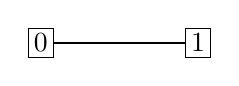
\begin{tikzpicture}[main_node/.style={rectangle,draw,minimum size=.5em,inner sep=2pt]}][!h]

		\node[main_node] (1) at (0,0){0};
		% [main_node] denotes the style defined at the beginning of the tikzpicture
		% (1) is the name of the node, use this name when drawing the edges
		% (0,0) denotes the position of the node
		% {0} denotes what the node is labeled
		\node[main_node] (2) at (2,0){1};

		\path[draw,thick]
    	(1) edge node {} (2)
    	% Draws edge from node 1 to node 2, if you want the edge labeled, put something in {}
    	;

	\end{tikzpicture}

	If you want this centered, put this code in a center environment

	\begin{center}
		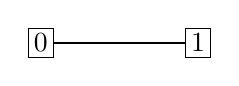
\begin{tikzpicture}[main_node/.style={rectangle,draw,minimum size=.5em,inner sep=2pt]}]

		\node[main_node] (1) at (0,0){0};
		\node[main_node] (2) at (2,0){1};

		\path[draw,thick]
    	(1) edge node {} (2)
    	;

		\end{tikzpicture}
	\end{center}

	If you want to label the graphs, use the figure environment

	\begin{figure}[!h]
		\begin{center}
			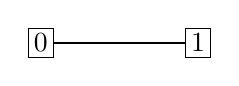
\begin{tikzpicture}[main_node/.style={rectangle,draw,minimum size=.5em,inner sep=2pt]}]

				\node[main_node] (1) at (0,0){0};
				\node[main_node] (2) at (2,0){1};

				\path[draw,thick]
    			(1) edge node {} (2)
    			;

			\end{tikzpicture}
		\end{center}
		\caption{$K_2$} % Note the inclusion of the caption package and the caption command in the preamble, that command gets rid of the caption labeling (it doesn't say fig 1 anymore)
	\end{figure}

	If you want to put multiple graphs in the same tikzpicture, use the scope parameter

	\begin{figure}[!h]
		\begin{center}
			\begin{tikzpicture}[main_node/.style={rectangle,draw,minimum size=.5em,inner sep=2pt]}]
				\begin{scope}[xshift=-3cm] %xshift shifts the graph relative to the center line
					\node[main_node] (1) at (0,0){0};
					\node[main_node] (2) at (2,0){1};

					\path[draw,thick]
    				(1) edge node {} (2)
    				;
    				\end{scope}


    				\begin{scope}[xshift=3cm]
    				\node[main_node] (1) at (0,0){00};
					\node[main_node] (2) at (2,0){10};
					\node[main_node] (3) at (2,2){11};
					\node[main_node] (4) at (0,2){01};

					\path[draw,thick]
    				(1) edge node {} (2)
    				(2) edge node {} (3)
    				(3) edge node {} (4)
    				(4) edge node {} (1)
    				;
    				\end{scope}
				\end{tikzpicture}
			\end{center}
			\caption{$Q_1$\hskip 160pt$Q_2$}
			% Note only one caption is placed, you have to add whitespace to put labels under each graph
	\end{figure}

	If you want to have nodes that are a solid color, add the fill parameter to the main\_node definition

	\begin{center}
		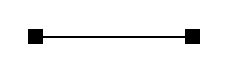
\begin{tikzpicture}[main_node/.style={rectangle,draw,fill=black,minimum size=.5em,inner sep=2pt]}]

		\node[main_node] (1) at (0,0){};
		\node[main_node] (2) at (2,0){};

		\path[draw,thick]
    	(1) edge node {} (2)
    	;

		\end{tikzpicture}
	\end{center}

\end{document}
